%%%%%%%%%%%%%%%%%%%%%%%%%%%%%%%%%%%%%%%%%%%%%%%%%%%%%%%%%%%%%%%%%%%%%%%%%%%%%%%%%%
 \begin{frame}[fragile]\frametitle{}
\begin{center}
{\Large Matrix}
\end{center}
\end{frame}


%%%%%%%%%%%%%%%%%%%%%%%%%%%%%%%%%%%%%%%%%%%%%%%%%%%%%%%%%%%
\begin{frame}[fragile]\frametitle{Meaning of a Matrix}

 \begin{itemize}
  \item Matrix is organization of data into rows and columns
  \item Example: columns can be various aspects of a person, such as height,weight, salary, etc, where as rows can represent different persons 
  \item This Excel sheet like data can be thought of as a Matrix (especially in Data Science, Machine Learning)
 \end{itemize}

\end{frame}



%%%%%%%%%%%%%%%%%%%%%%%%%%%%%%%%%%%%%%%%%%%%%%%%%%%%%%%%%%%
 \begin{frame}[fragile] \frametitle{Matrix }
A matrix is an array of numbers that can be arranged into rows
and columns. We generally name matrices with a capital letter.

$A = \begin{bmatrix}
  1 & 2 & 3 \\
  4 & 5 & 6
 \end{bmatrix}$
 
\begin{lstlisting}
 import numpy as np

A = np.array([[1,2,3],
              [4,5,6]])
print (A)

[[1 2 3]
 [4 5 6]]
\end{lstlisting}


\end{frame}

%%%%%%%%%%%%%%%%%%%%%%%%%%%%%%%%%%%%%%%%%%%%%%%%%%%%%%%%%%%
  \begin{frame}[fragile]\frametitle{Matrix}
\textbf{Definition}
A matrix with $m$ rows and $n$ columns is referred to as an $m \times n$ matrix.
The number of rows always comes before the number of columns.
%Thus the matrices above are $2 \times 2$ and $2 \times 3$ respectively.

$A = \begin{bmatrix}
  a_{1,1} & a_{1,2} & a_{1,3} \\
  a_{2,1} & a_{2,2} & a_{2,3}
 \end{bmatrix}$
 
\begin{lstlisting}
import numpy as np

M = np.matrix([[1,2,3],
               [4,5,6]])
print (M)

[[1 2 3]
 [4 5 6]] 
\end{lstlisting}


\end{frame}


%%%%%%%%%%%%%%%%%%%%%%%%%%%%%%%%%%%%%%%%%%%%%%%%%%%%%%%%%%%
 \begin{frame}[fragile] \frametitle{Matrix Addition}
 You can
add or subtract matrices of the same size by simply adding or subtracting the
corresponding elements in the two matrices. 

\begin{center}
\includegraphics[width=0.5\linewidth,keepaspectratio]{mat1}
\end{center}

$\begin{bmatrix}1 & 2 & 3 \\4 & 5 & 6\end{bmatrix}+ \begin{bmatrix}6 & 5 & 4 \\3 & 2 & 1\end{bmatrix} = \begin{bmatrix}7 & 7 & 7 \\7 & 7 & 7\end{bmatrix}$
\end{frame}

%%%%%%%%%%%%%%%%%%%%%%%%%%%%%%%%%%%%%%%%%%%%%%%%%%%%%%%%%%%
  \begin{frame}[fragile]\frametitle{Matrix Addition}
 
\begin{lstlisting}
import numpy as np

A = np.array([[1,2,3],
              [4,5,6]])
B = np.array([[6,5,4],
              [3,2,1]])
print(A + B)

[[7 7 7]
 [7 7 7]]
\end{lstlisting}

\end{frame}

%%%%%%%%%%%%%%%%%%%%%%%%%%%%%%%%%%%%%%%%%%%%%%%%%%%%%%%%%%%
  \begin{frame}[fragile]\frametitle{Matrix Subtraction}
 
 $\begin{bmatrix}1 & 2 & 3 \\4 & 5 & 6\end{bmatrix}- \begin{bmatrix}6 & 5 & 4 \\3 & 2 & 1\end{bmatrix} = \begin{bmatrix}-5 & -3 & -1 \\1 & 3 & 5\end{bmatrix}$
\begin{lstlisting}
import numpy as np

A = np.array([[1,2,3],
              [4,5,6]])
B = np.array([[6,5,4],
              [3,2,1]])
print(A - B)

[[-5 -3 -1]
 [ 1  3  5]]
\end{lstlisting}

\end{frame}


%%%%%%%%%%%%%%%%%%%%%%%%%%%%%%%%%%%%%%%%%%%%%%%%%%%%%%%%%%%
\begin{frame}[fragile]\frametitle{The Transpose of a Matrix}
\textbf{Definition}
The transpose of a $m\times n$ matrix $A$ is the matrix $A^{T}$ 
having $(i,j)$-entry $a_{ji}$.  That is,
$$(A^{T})_{i j} = a_{j i}.$$



\textbf{Example}
For example, 
$ A = \left[ \begin{array}{rrr}
      1 & 2 & 3 \\
      4 & 5 & 6
     \end{array}\right]$
has transpose  
$A^T = \left[\begin{array}{rrr}
        1 & 4 \\ 
        2 & 5 \\
        3 & 6
       \end{array}\right]$.



\textbf{Note}
The rows of $A$ become the columns of $A^T$ and vice versa.

\end{frame}


%%%%%%%%%%%%%%%%%%%%%%%%%%%%%%%%%%%%%%%%%%%%%%%%%%%%%%%%%%%
\begin{frame}[fragile]\frametitle{Meaning of a Matrix Multiplication}

 \begin{itemize}
  \item Matrix is organization of data into rows and columns
  \item Example: columns can be various aspects of a person, such as height,weight, salary, etc, where as rows can represent different persons 
  \item This Excel sheet like data can be thought of as a Matrix (especially in Data Science, Machine Learning)
  \item If you have another matrix like this, what is the meaning of their multiplication?
  \item Geometrically: say first matrix represents points of a shape, a polygon, where each row is a point, and each column represents X, Y, Z coordinates.
  \item Second matrix is typically a Homogeneous transformation matrix, such as rotation,  when multiplied gets rotated shape.
 \end{itemize}

\end{frame}

%%%%%%%%%%%%%%%%%%%%%%%%%%%%%%%%%%%%%%%%%%%%%%%%%%%%%%%%%%%
\begin{frame}[fragile]\frametitle{Matrix Multiplication Rules}
\textbf{Theorem}  Let $A$ and $B$ be matrices whose sizes are appropriate for the following 
sums and products to be defined
 \begin{itemize}
  \item $(A^T)^T = A$
\item $(A+B)^T = A^T + B^T$.
\item For any scalar $r$, $(rA)^T=rA^T$.
\item $(AB)^T = B^T A^T$
 \end{itemize}


\end{frame}


%%%%%%%%%%%%%%%%%%%%%%%%%%%%%%%%%%%%%%%%%%%%%%%%%%%%%%%%%%%
\begin{frame}[fragile]\frametitle{Example}
  
$A = \begin{bmatrix} 1 & 2 \\ 3 & 4 \end{bmatrix}$, and $B= 
\begin{bmatrix}
 5 & 1 & -1 \\
 1 & 2 & 2 
\end{bmatrix}$
then 
\[
 AB = \begin{bmatrix}
       7 & 5 & 3 \\
       9 & 11 & 5
      \end{bmatrix}
\qquad 
(AB)^T = \begin{bmatrix} 7 & 9 \\
          5 & 11 \\ 3 & 5
         \end{bmatrix} = B^T A^T
\]
but $A^T$ is $2\times 2$ and $B^T$ is $3 \times 2$, so $A^TB^T$ isn't even defined.

\end{frame}


%
%
%
%
%  \begin{frame}[fragile]
%\textbf{Definition}
%Suppose that $T: \mathbb R^n \longrightarrow \mathbb R^m$ is linear.   We will say that 
%$T$ is invertible if for every $\vec{b} \in \mathbb R^m$
%there is exactly one $\vec{x} \in \mathbb R^n$ so that $T(\vec{x})= \vec{b}$.
%
%
%
%\textbf{Note}
%If $T$ is invertible, this means that $T$ is onto 
%(every equation can be solved: hence $m\leq n$) and $T$ is 1-1 (every equation 
%has at most one solution: hence $n \leq m$).  
%
%
%Thus $n=m$ and  an invertible linear transformation has a matrix which must be square.  
%
%
%
%
%\textbf{Questions}
%\begin{itemize}
%\item Which square matrices are invertible? 
%\item What does it mean for a square matrix to be invertible?
%\end{itemize}
%
%\end{frame}
%
%
%
%
%
%
%  \begin{frame}[fragile]
%\textbf{Facts}
%Suppose that $T: \mathbb R^n \longrightarrow \mathbb R^n$ is an invertible linear transformation: then we
%can define $S : \mathbb R^n \longrightarrow \mathbb R^n$ so that $T\vec{x} = \vec{u}$ if and 
%only if $\vec{x}= S(\vec{u})$.  Furthermore, for every vector 
%$\vec{x} \in \mathbb R^n$,  $S(T(\vec{x}))=\vec{x}$, and 
%for every $\vec{u} \in \mathbb R^n$, $T(S(\vec{u}))= \vec{u}$.
%
%
%
%\textbf{Facts}
%It turns out that $S$ must also be linear. 
%\end{frame}
%
%
%
%
%
%  \begin{frame}[fragile]
%\textbf{Proof}
%We'll assume that $T(\vec{x})= \vec{u}$
% and $T(\vec{y})=\vec{v}$.  Then $S(\vec{u}) = \vec{x} $
%and $S(\vec{v} ) =\vec{y}$.
%
%
%Note that
% $S(T(r\vec{x})) = r\vec{x}$,
%so  we get
% \[
%S(r \vec{u}) = S(r T(\vec{x})) = S(T(r \vec{x}))= r\vec{x}
% = r S(\vec{u} ) 
%   \]
%so that $S$ commutes with scalar addition.
%
%
%Likewise,
%\[
% S(\vec{u} + \vec{v}) = 
%S( T(\vec{x}) + T(\vec{y}) ) =
%S ( T (\vec{x} + \vec{y} )) =
%(\vec{x} + \vec{y}) =
%S(\vec{u}) + S(\vec{v})
%\]
% so that $S$ commutes with addition.  
% 
% Thus $S$ is linear.
%
%\end{frame}
%
%
%
%
%
%
%  \begin{frame}[fragile]
%\textbf{Note}
%We see that if $T$ is an invertible linear transformation from $\mathbb R^n$ to $\mathbb R^n$, then so is $S$.  \\ 
%Hence we can represent $T$ by a square matrix $A$ and $S$ by a square matrix $B$.
%
%
%Then $S(T(\vec{x}))= \vec{x}$ for all $\vec{x}$ means that 
%$BA \vec{x}= \vec{x}$ for every $\vec{x}$.  \\ 
%
%In particular, if 
%$C=BA$, then we have $C \vec{e}_j = \vec{e}_j$, so that we obtain that 
%$C$ must be the identity matrix $I_n$.  \\ 
%
%Similarly, $T(S(\vec{u})) = \vec{u}$ for every $\vec{u}$, and hence
%$AB=I_n$ is also the identity matrix.
%
%\end{frame}



%%%%%%%%%%%%%%%%%%%%%%%%%%%%%%%%%%%%%%%%%%%%%%%%%%%%%%%%%%%
 \begin{frame}[fragile] \frametitle{Matrix Transpose}
Exchange rows and columns

\begin{center}
\includegraphics[width=0.5\linewidth,keepaspectratio]{mat2}
\end{center}
\end{frame}

%%%%%%%%%%%%%%%%%%%%%%%%%%%%%%%%%%%%%%%%%%%%%%%%%%%%%%%%%%%
\begin{frame}[fragile]\frametitle{Matrix Transpose}
 
$\begin{bmatrix}1 & 2 & 3 \\4 & 5 & 6\end{bmatrix}^{T} = \begin{bmatrix}1 & 4\\2 & 5\\3 & 6 \end{bmatrix}$

\begin{lstlisting}
import numpy as np

A = np.array([[1,2,3],
              [4,5,6]])
print(A.T)

[[1 4]
 [2 5]
 [3 6]]
\end{lstlisting}

\end{frame}

%%%%%%%%%%%%%%%%%%%%%%%%%%%%%%%%%%%%%%%%%%%%%%%%%%%%%%%%%%%
 \begin{frame}[fragile] \frametitle{Matrix Multiplication}
 Here are the cases to consider:
\begin{itemize}
\item Scalar multiplication, which is
multiplying a matrix by a single number
\item Element wise matrix multiplication (rarely used, called Hadamard multiplication, shown with circle instead of dot)
\item Dot product matrix multiplication, or
multiplying a matrix by another matrix.
\end{itemize}

\end{frame}


%%%%%%%%%%%%%%%%%%%%%%%%%%%%%%%%%%%%%%%%%%%%%%%%%%%%%%%%%%%
 \begin{frame}[fragile] \frametitle{Matrix Scalar Multiplication}
To multiply a matrix by a scalar value, you just multiply each element by the scalar to produce a new matrix:

$2 \times \begin{bmatrix}1 & 2 & 3 \\4 & 5 & 6\end{bmatrix} = \begin{bmatrix}2 & 4 & 6 \\8 & 10 & 12\end{bmatrix}$


\begin{lstlisting}
import numpy as np
import numpy as np

A = np.array([[1,2,3],
              [4,5,6]])
print(2 * A)

[[ 2  4  6]
 [ 8 10 12]]
\end{lstlisting}

\end{frame}

%%%%%%%%%%%%%%%%%%%%%%%%%%%%%%%%%%%%%%%%%%%%%%%%%%%%%%%%%%%
  \begin{frame}[fragile]\frametitle{Matrix Multiplication Defined}
\textbf{Definition}
If $A$ is an $m \times n$ matrix, and if $B=[\vec{b}_1,\vec{b}_2 \dots, \vec{b}_p]$ is a $n\times p$ matrix, then the matrix product
$AB$ is the following $m \times p$ matrix.
\[
 AB = [ A \vec{b}_1 \ \ \  A \vec{b}_2 \ \ \  \dots 
\ \ \  A \vec{b}_p ]
\]



\textbf{Example}
Let $A =\left[\begin{array}{rr} 1& 2 \\ -2 & 3\end{array}\right]$ and let $B=\left[\begin{array}{rrr} 3 & -1 & 6 \\ 7& 5& 3\end{array}\right]$.  Compute $AB$.

\end{frame}





%%%%%%%%%%%%%%%%%%%%%%%%%%%%%%%%%%%%%%%%%%%%%%%%%%%%%%%%%%%
  \begin{frame}[fragile]\frametitle{Multiplying Matrices}
\textbf{Row-Column Rule}
If $A$ is  $m \times n$ and if $B$ is $n\times p$ the $(i,j)$-entry of $AB$ is 
given by 
\[
 (AB)_{ij} = \sum_{k=1}^n a_{ik} b_{kj}
\]



\textbf{Note}
$\mbox{Row}_i(AB) = \mbox{Row}_i(A) \cdot B$.

\end{frame}


% %%%%%%%%%%%%%%%%%%%%%%%%%%%%%%%%%%%%%%%%%%%%%%%%%%%%%%%%%%%
 % \begin{frame}[fragile] \frametitle{Matrix Dot Product Multiplication}
% \begin{itemize}
% \item  Multiplying each of the elements in each row of the first matrix by each of the elements in each column of the second matrix and adding the results.
% \item  $\begin{bmatrix}1 & 2 & 3 \\4 & 5 & 6\end{bmatrix} \cdot \begin{bmatrix}9 & 8 \\ 7 & 6 \\ 5 & 4\end{bmatrix}$
% \item  We first take the dot product of the first row of the first matrix (1,2,3) and the first column of the second matrix (9,7,5):
% $(1,2,3) \cdot (9,7,5) = (1 \times 9) + (2 \times 7) + (3 \times 5) = 38$
% \item $\begin{bmatrix}38 & ?\\? & ?\end{bmatrix}$
% \end{itemize}
% \end{frame}

% %%%%%%%%%%%%%%%%%%%%%%%%%%%%%%%%%%%%%%%%%%%%%%%%%%%%%%%%%%%
 % \begin{frame}[fragile] \frametitle{Matrix Dot Product Multiplication}
% \begin{itemize}
% \item  Now we can take the dot product of the first row of the first matrix and the second column of the second matrix:
% \item $(1,2,3) \cdot (8,6,4) = (1 \times 8) + (2 \times 6) + (3 \times 4) = 32$
% \item $\begin{bmatrix}38 & 32\\? & ?\end{bmatrix} $
% \item Now we can repeat this process for the second row of the first matrix and the first column of the second matrix: 
% $(4,5,6) \cdot (9,7,5) = (4 \times 9) + (5 \times 7) + (6 \times 5) = 101$
% \item $\begin{bmatrix}38 & 32\\101 & ?\end{bmatrix}$
% \end{itemize}
% \end{frame}

% %%%%%%%%%%%%%%%%%%%%%%%%%%%%%%%%%%%%%%%%%%%%%%%%%%%%%%%%%%%
 % \begin{frame}[fragile] \frametitle{Matrix Dot Product Multiplication}
% \begin{itemize}
% \item  Finally, we get the dot product for the second row of the first matrix and the second column of the second matrix:
% \item $(4,5,6) \cdot (8,6,4) = (4 \times 8) + (5 \times 6) + (6 \times 4) = 86$
% \item Giving us:
% \item $\begin{bmatrix}38 & 32\\101 & 86\end{bmatrix}$
% \end{itemize}
% \end{frame}

% %%%%%%%%%%%%%%%%%%%%%%%%%%%%%%%%%%%%%%%%%%%%%%%%%%%%%%%%%%%
 % \begin{frame}[fragile] \frametitle{Matrix Dot Product Multiplication}

% \begin{lstlisting}
% import numpy as np

% A = np.array([[1,2,3],
              % [4,5,6]])
% B = np.array([[9,8],
              % [7,6],
              % [5,4]])
% print(np.dot(A,B))
% print(A @ B)

% [[ 38  32]
 % [101  86]]
% [[ 38  32]
 % [101  86]]
% \end{lstlisting}

% \end{frame}

% %%%%%%%%%%%%%%%%%%%%%%%%%%%%%%%%%%%%%%%%%%%%%%%%%%%%%%%%%%%
  % \begin{frame}[fragile]
% \textbf{Definition}
% We define the $m\times m$ identity matrix as
% \begin{equation*}
% I_m =[\vec{e}_1, \vec{e}_2, \dots \vec{e}_m] = \left[\begin{array}{rrrrr}  1& 0 &  \dots & 0 \\  0& 1&  \dots & 0 \\ \vdots& \vdots &  \ddots & \vdots \\
                                                                                                                % 0& 0&  \dots & 1 \end{array}\right].
% \end{equation*}



% \textbf{Theorem}
 % With $A$, $B$ and $C$ appropriately sized matrices and $r$ a scalar
% \begin{itemize}
 % \item $(AB)C = A(BC)$
% \item $A(B+C) = AB + AC$
% \item $(B+C)A = BA + CA$
% \item $r(AB) = (rA)B = A(rB)$ 
% \item $I_m A = A = A I_n$
% \end{itemize}

% \end{frame}




% %%%%%%%%%%%%%%%%%%%%%%%%%%%%%%%%%%%%%%%%%%%%%%%%%%%%%%%%%%%
  % \begin{frame}[fragile]\frametitle{Properties Not held by Matrix Multiplication}
% \textbf{Example}
% Let $A=\left[\begin{array}{rr} 1& 2 \\ 5 & 10 \end{array}\right]$.  \\ 
% Let $B=\left[\begin{array}{rr}  2 & 6 \\ -1 & -3 \end{array}\right]$.   \\
% Compute $AB$, $BA$, and $A\cdot 0$.



% \textbf{Note}
% \begin{itemize}
% \item It is {\bf NOT} in general true that $AB=BA$.
% \item It is {\bf NOT} in general true when $AC=AB$ that $C=B$.
% \end{itemize}


% \end{frame}

% %%%%%%%%%%%%%%%%%%%%%%%%%%%%%%%%%%%%%%%%%%%%%%%%%%%%%%%%%%%
  % \begin{frame}[fragile]\frametitle{Exponents}
% \textbf{Definition}
% We define non negative powers of an $m\times m$ matrix as follows. 
% \begin{equation*}
% A^0=I_m, \qquad A^1=A, \qquad A^n=A^{n-1}A \qquad\mbox{for $n>1$}.
% \end{equation*}


% \textbf{Example}
% Let $A=\left[\begin{array}{rr} 1 & 2 \\ 0 & 1\end{array}\right]$.  Compute $A^3$.

% \end{frame}


% %%%%%%%%%%%%%%%%%%%%%%%%%%%%%%%%%%%%%%%%%%%%%%%%%%%%%%%%%%%
 % \begin{frame}[fragile] \frametitle{Matrix Division}
% \begin{itemize}
% \item  You can't actually divide by a matrix; but when you want to divide matrices, you can take advantage of the fact that division by a given number is the same as multiplication by the reciprocal of that number. For example: $6 \div 3 = \frac{1}{3}\times 6$
% \item Reciprocal can be treated as inverse.
% \item So $A \div B = A \cdot B^{-1}$
% \end{itemize}
% \end{frame}


% %%%%%%%%%%%%%%%%%%%%%%%%%%%%%%%%%%%%%%%%%%%%%%%%%%%%%%%%%%%
% \begin{frame}[fragile] \frametitle{Matrix Inversion}

% \textbf{Definition}
% \begin{itemize}
% \item  An $n\times n$ matrix $A$ is {\em invertible} if there exists a $n\times n$ matrix $B$
% so that $AB = I_n = BA$.  
% \item  $B$ is called the {\em inverse} of $A$ and is denoted by $A^{-1}$.   
% \item  A matrix which is not invertible is said to be {\em singular}.
% \end{itemize}
% \end{frame}


% %%%%%%%%%%%%%%%%%%%%%%%%%%%%%%%%%%%%%%%%%%%%%%%%%%%%%%%%%%%
% \begin{frame}[fragile]\frametitle{The Speical Case of $2\times 2$ Matrices}


% \textbf{Definition}
 % Let $A= \begin{bmatrix} a & b \\ c& d \end{bmatrix}$.  We define (and this only works for
% $2\times 2$ matrices) the determinant of $A$ to be the quantity $$\det(A) = ad-bc.$$

% \textbf{Theorem}
 % Let $A = \begin{bmatrix} a & b \\ c& d \end{bmatrix}$.  Then $A$ is invertible if and only
% if $\det(A)$ is non-zero, in which case
% \[
 % A^{-1} = \frac{1}{\det(A)} \left[\begin{array}{rr} d & -b \\ -c& a \end{array}\right]. 
% \]
% If $\det(A)=0$ then $A$ is {\em singular}.

% \end{frame}

% %%%%%%%%%%%%%%%%%%%%%%%%%%%%%%%%%%%%%%%%%%%%%%%%%%%%%%%%%%%
% \begin{frame}[fragile]
% \textbf{Theorem}
 % If $A$ is an invertible $m\times m$ matrix, 
% then for every $\vec{b}\in \mathbb R^n$, the equation 
% $A \vec{x}=\vec{b}$ has a unique solution, 
% namely $\vec{x} = A^{-1} \vec{b}$.


% \textbf{Proof}
% \ \\
% \textbf{Theorem}
% \begin{itemize}
 % \item  If $A$ is invertible, then so is $A^{-1}$, and $(A^{-1})^{-1} = A$.
% \item If $A$ and $B$ are invertible $n \times n$ matrices  then so is $AB$, and $(AB)^{-1} = B^{-1}A^{-1}$.
% \item If $A$ is invertible, then so is $A^{T}$, and $(A^T)^{-1} = (A^{-1})^T$.
% \end{itemize}


% \textbf{Proof}
% \ \\


% \end{frame}



% %%%%%%%%%%%%%%%%%%%%%%%%%%%%%%%%%%%%%%%%%%%%%%%%%%%%%%%%%%%
 % \begin{frame}[fragile] \frametitle{Matrix Inversion}
% \begin{itemize}
% \item For a 2x2 matrix, you can follow this formula:
% \item $\begin{bmatrix}a & b\\c & d\end{bmatrix}^{-1} = \frac{1}{ad-bc}  \begin{bmatrix}d & -b\\-c & a\end{bmatrix}$
% \item What happened there?
% \begin{itemize}

% \item We swapped the positions of a and d
% \item We changed the signs of b and c
% \item We multiplied the resulting matrix by 1 over the determinant of the matrix (ad-bc)
% \end{itemize}

% \end{itemize}
% \end{frame}

% %%%%%%%%%%%%%%%%%%%%%%%%%%%%%%%%%%%%%%%%%%%%%%%%%%%%%%%%%%%
 % \begin{frame}[fragile] \frametitle{Matrix Inversion}
% \begin{itemize}
% \item $\begin{bmatrix}6 & 2\\1 & 2\end{bmatrix}^{-1} = \frac{1}{(6\times2)-(2\times1)}  \begin{bmatrix}2 & -2\\-1 & 6\end{bmatrix}$
% \item $\begin{bmatrix}6 & 2\\1 & 2\end{bmatrix}^{-1} = \frac{1}{10}  \begin{bmatrix}2 & -2\\-1 & 6\end{bmatrix}$
% \item $\begin{bmatrix}6 & 2\\1 & 2\end{bmatrix}^{-1} = \begin{bmatrix}0.2 & -0.2\\-0.1 & 0.6\end{bmatrix}$
% \item To Check:
% $\begin{bmatrix}6 & 2\\1 & 2\end{bmatrix} \cdot \begin{bmatrix}0.2 & -0.2\\-0.1 & 0.6\end{bmatrix} = \begin{bmatrix}(6\times0.2)+(2\times-0.1) & (6\times-0.2)+(2\times0.6)\\(1\times0.2)+(2\times-0.1) & (1\times-0.2)+(2\times0.6)\end{bmatrix} = \begin{bmatrix}1 & 0\\0 & 1\end{bmatrix}$
% \end{itemize}
% \end{frame}

% %%%%%%%%%%%%%%%%%%%%%%%%%%%%%%%%%%%%%%%%%%%%%%%%%%%%%%%%%%%
 % \begin{frame}[fragile] \frametitle{Matrix Inversion}

% \begin{lstlisting}
% import numpy as np

% B = np.array([[6,2],
              % [1,2]])

% print(np.linalg.inv(B))

% [[ 0.2 -0.2]
 % [-0.1  0.6]]
% \end{lstlisting}

% \end{frame}


% %%%%%%%%%%%%%%%%%%%%%%%%%%%%%%%%%%%%%%%%%%%%%%%%%%%%%%%%%%%
 % \begin{frame}[fragile] \frametitle{Matrix Inversion}
 % For larger matrices, the process to calculate the inverse is more complex. Let's explore an example based on the following matrix:
 
 % $\begin{bmatrix}4 & 2 & 2\\6 & 2 & 4\\2 & 2 & 8\end{bmatrix}$
 

% \end{frame}


% %%%%%%%%%%%%%%%%%%%%%%%%%%%%%%%%%%%%%%%%%%%%%%%%%%%%%%%%%%%
 % \begin{frame}[fragile] \frametitle{Matrix Inversion}
% Create a matrix of minors by calculating the determinant for each element in the matrix based on the elements that are not in the same row or column; like this:
 
% \begin{itemize}

% \item $\begin{bmatrix}\color{blue}4 & \color{lightgray}2 & \color{lightgray}2\\\color{lightgray}6 & \color{red}2 & \color{red}4\\\color{lightgray}2 & \color{red}2 & \color{red}8\end{bmatrix}\;\;\;\;(2\times8) - (4\times2) = 8\;\;\;\;\begin{bmatrix}8 & \color{lightgray}? & \color{lightgray}?\\\color{lightgray}? & \color{lightgray}? & \color{lightgray}?\\\color{lightgray}? & \color{lightgray}? & \color{lightgray}?\end{bmatrix} $
% \item $\begin{bmatrix}\color{lightgray}4 & \color{blue}2 & \color{lightgray}2\\\color{red}6 & \color{lightgray}2 & \color{red}4\\\color{red}2 & \color{lightgray}2 & \color{red}8\end{bmatrix}\;\;\;\;(6\times8) - (4\times2) = 40\;\;\;\;\begin{bmatrix}8 & 40 & \color{lightgray}?\\\color{lightgray}? & \color{lightgray}? & \color{lightgray}?\\\color{lightgray}? & \color{lightgray}? & \color{lightgray}?\end{bmatrix}$
% \end{itemize}
% \end{frame}

% %%%%%%%%%%%%%%%%%%%%%%%%%%%%%%%%%%%%%%%%%%%%%%%%%%%%%%%%%%%
 % \begin{frame}[fragile] \frametitle{Matrix Inversion}

% \begin{itemize}
% \item $\begin{bmatrix}\color{lightgray}4 & \color{lightgray}2 & \color{blue}2\\\color{red}6 & \color{red}2 & \color{lightgray}4\\\color{red}2 & \color{red}2 & \color{lightgray}8\end{bmatrix}\;\;\;\;(6\times2) - (2\times2) = 8\;\;\;\;\begin{bmatrix}8 & 40 & 8\\\color{lightgray}? & \color{lightgray}? & \color{lightgray}?\\\color{lightgray}? & \color{lightgray}? & \color{lightgray}?\end{bmatrix} $
% \item $\begin{bmatrix}\color{lightgray}4 & \color{red}2 & \color{red}2\\\color{blue}6 & \color{lightgray}2 & \color{lightgray}4\\\color{lightgray}2 & \color{red}2 & \color{red}8\end{bmatrix}\;\;\;\;(2\times8) - (2\times2) = 12\;\;\;\;\begin{bmatrix}8 & 40 & 8\\12 & \color{lightgray}? & \color{lightgray}?\\\color{lightgray}? & \color{lightgray}? & \color{lightgray}?\end{bmatrix}$
% \item $\ldots$
% \item $\begin{bmatrix}\color{red}4 & \color{red}2 & \color{lightgray}2\\\color{red}6 & \color{red}2 & \color{lightgray}4\\\color{lightgray}2 & \color{lightgray}2 & \color{blue}8\end{bmatrix}\;\;\;\;(4\times2) - (2\times6) = -4\;\;\;\;\begin{bmatrix}8 & 40 & 8\\12 & 28 & 4\\4 & 4 & -4\end{bmatrix}$
% \end{itemize}
% \end{frame}

% %%%%%%%%%%%%%%%%%%%%%%%%%%%%%%%%%%%%%%%%%%%%%%%%%%%%%%%%%%%
 % \begin{frame}[fragile] \frametitle{Matrix Inversion}
% Apply cofactors to the matrix by switching the sign of every alternate element in the matrix of minors:


% $\begin{bmatrix}8 & -40 & 8\\-12 & 28 & -4\\4 & -4 & -4\end{bmatrix}$


% Adjugate by transposing elements diagonally:

% $\begin{bmatrix}8 & \color{green}-\color{green}1\color{green}2 & \color{orange}4\\\color{green}-\color{green}4\color{green}0 & 28 & \color{purple}-\color{purple}4\\\color{orange}8 & \color{purple}-\color{purple}4 & -4\end{bmatrix} $
% \end{frame}


% %%%%%%%%%%%%%%%%%%%%%%%%%%%%%%%%%%%%%%%%%%%%%%%%%%%%%%%%%%%
 % \begin{frame}[fragile] \frametitle{Matrix Inversion}

 % Multiply by 1/determinant of the original matrix. To find this, multiply each of the top row elements by their corresponding minor determinants (which we calculated earlier in the matrix of minors), and then subtract the second from the first and add the third:
 
 % $Determinant = (4 \times 8) - (2 \times 40) + (2 \times 8) = -32$
 
 
 % $\frac{1}{-32}\begin{bmatrix}8 & -12 & 4\\-40 & 28 & -4\\8 & -4 & -4\end{bmatrix} =  \begin{bmatrix}-0.25 & 0.375 & -0.125\\1.25 & -0.875 & 0.125\\-0.25 & 0.125 & 0.125\end{bmatrix}$
% \end{frame}

% %%%%%%%%%%%%%%%%%%%%%%%%%%%%%%%%%%%%%%%%%%%%%%%%%%%%%%%%%%%
 % \begin{frame}[fragile] \frametitle{Matrix Inversion}
% To Test:

% $\begin{bmatrix}4 & 2 & 2\\6 & 2 & 4\\2 & 2 & 8\end{bmatrix} \cdot \begin{bmatrix}-0.25 & 0.375 & -0.125\\1.25 & -0.875 & 0.125\\-0.25 & 0.125 & 0.125\end{bmatrix}$

% $= \begin{bmatrix}(4\times-0.25)+(2\times1.25)+(2\times-0.25) & (4\times0.375)+(2\times-0.875)+(2\times0.125) & (4\times-0.125)+(2\times-0.125)+(2\times0.125)\\(6\times-0.25)+(2\times1.25)+(4\times-0.25) & (6\times0.375)+(2\times-0.875)+(4\times0.125) & (6\times-0.125)+(2\times-0.125)+(4\times0.125)\\(2\times-0.25)+(2\times1.25)+(8\times-0.25) & (2\times0.375)+(2\times-0.875)+(8\times0.125) & (2\times-0.125)+(2\times-0.125)+(8\times0.125)\end{bmatrix}$

% $= \begin{bmatrix}1 & 0 & 0\\0 & 1 & 0\\0 & 0 & 1\end{bmatrix}$

 % \end{frame}

% %%%%%%%%%%%%%%%%%%%%%%%%%%%%%%%%%%%%%%%%%%%%%%%%%%%%%%%%%%%
 % \begin{frame}[fragile] \frametitle{Matrix Inversion}

% \begin{lstlisting}
% import numpy as np

% B = np.array([[4,2,2],
              % [6,2,4],
              % [2,2,8]])

% print(np.linalg.inv(B))

% [[-0.25   0.375 -0.125]
 % [ 1.25  -0.875  0.125]
 % [-0.25   0.125  0.125]]
% \end{lstlisting}

% \end{frame}

%%%%%%%%%%%%%%%%%%%%%%%%%%%%%%%%%%%%%%%%%%%%%%%%%%%%%%%%%%%
  \begin{frame}[fragile]\frametitle{Matrix Operations}
Additions
\begin{itemize}
\item Commutative: $A + B = B + A$
\item Associative: $A + (B + C) = (A + B) + C$
\end{itemize}
Multiplication
\begin{itemize}
\item Scalar : $sA$: multiplying all elements by $s$
\item Commutative: $AB \neq BA$
\item Associative: $A(BC)  =  (AB)C$
\item Distributive: $A(B + C)  =  AB + AC$
\item Identity: $ I_mA_{mn}  =  A_{mn}I_n  =  A$
\end{itemize}
\end{frame}

% %%%%%%%%%%%%%%%%%%%%%%%%%%%%%%%%%%%%%%%%%%%%%%%%%%%%%%%%%%%%%%%%%%%%%%%%%%%%%%%%%%
  % \begin{frame}[fragile]\frametitle{}
% \begin{center}
% {\Large Matrix Transformations}
% \end{center}
% \end{frame}

% %%%%%%%%%%%%%%%%%%%%%%%%%%%%%%%%%%%%%%%%%%%%%%%%%%%%%%%%%%%
 % \begin{frame}[fragile] \frametitle{Linear Transformations}

% \begin{itemize}

% \item You can manipulate a vector by multiplying it with a matrix. 
% \item The matrix acts a function that operates on an input vector to produce a vector output. 
% \item Specifically, matrix multiplications of vectors are linear transformations that transform the input vector into the output vector.
% \end{itemize}

% \end{frame}


% %%%%%%%%%%%%%%%%%%%%%%%%%%%%%%%%%%%%%%%%%%%%%%%%%%%%%%%%%%%
 % \begin{frame}[fragile] \frametitle{Linear Transformations}

% \begin{itemize}

% \item $A = \begin{bmatrix}2 & 3\\5 & 2\end{bmatrix} \;\;\;\; \vec{v} = \begin{bmatrix}1\\2\end{bmatrix}$
% \item We can define a transformation T like this:
% \item $T(\vec{v}) = A\vec{v}$
% \item $\begin{bmatrix}2 & 3\\5 & 2\end{bmatrix} \cdot  \begin{bmatrix}1\\2\end{bmatrix} = \begin{bmatrix}8\\9\end{bmatrix}$
% \end{itemize}

% \end{frame}


% %%%%%%%%%%%%%%%%%%%%%%%%%%%%%%%%%%%%%%%%%%%%%%%%%%%%%%%%%%%
 % \begin{frame}[fragile] \frametitle{Transformations of Magnitude and Amplitude}
% When you multiply a vector by a matrix, you transform it in at least one of the following two ways:
% \begin{itemize}

% \item Scale the length (magnitude) of the matrix to make it longer or shorter
% \item Change the direction (amplitude) of the matrix
% \end{itemize}

% \end{frame}

% %%%%%%%%%%%%%%%%%%%%%%%%%%%%%%%%%%%%%%%%%%%%%%%%%%%%%%%%%%%
 % \begin{frame}[fragile] \frametitle{Transformations of Magnitude and Amplitude}
% When you multiply a vector by a matrix, you transform it in at least one of the following two ways:
% \begin{itemize}

% \item $A = \begin{bmatrix}2 & 0\\0 & 2\end{bmatrix} \;\;\;\; \vec{v} = \begin{bmatrix}1\\0\end{bmatrix}$
% \item $\begin{bmatrix}2 & 0\\0 & 2\end{bmatrix} \cdot  \begin{bmatrix}1\\0\end{bmatrix} = \begin{bmatrix}2\\0\end{bmatrix}$
% \end{itemize}

% \end{frame}

% %%%%%%%%%%%%%%%%%%%%%%%%%%%%%%%%%%%%%%%%%%%%%%%%%%%%%%%%%%%
 % \begin{frame}[fragile] \frametitle{Transformations of Magnitude and Amplitude}
% \begin{lstlisting}
% import numpy as np
% import matplotlib.pyplot as plt
% v = np.array([1,0])
% A = np.array([[2,0],
              % [0,2]])
% t = A@v
% print (t)
% # Plot v and t
% vecs = np.array([t,v])
% origin = [0], [0]
% plt.axis('equal')
% plt.grid()
% plt.ticklabel_format(style='sci', axis='both', scilimits=(0,0))
% plt.quiver(*origin, vecs[:,0], vecs[:,1], color=['blue', 'orange'], scale=10)
% plt.show()
% \end{lstlisting}
% [2 0]
% \end{frame}

% %%%%%%%%%%%%%%%%%%%%%%%%%%%%%%%%%%%%%%%%%%%%%%%%%%%%%%%%%%%
 % \begin{frame}[fragile] \frametitle{Affine Transformations}


% \begin{center}
% \includegraphics[width=0.5\linewidth,keepaspectratio]{vec7}
% \end{center}
% The original vector v is shown in orange, and the transformed vector t is shown in blue - note that t has the same direction (amplitude) as v but a greater length (magnitude).
 
% \end{frame}


% %%%%%%%%%%%%%%%%%%%%%%%%%%%%%%%%%%%%%%%%%%%%%%%%%%%%%%%%%%%
 % \begin{frame}[fragile] \frametitle{Affine Transformations}
% An Affine transformation multiplies a vector by a matrix and adds an offset vector, sometimes referred to as bias; like this:

% \begin{itemize}

% \item $T(\vec{v}) = A\vec{v} + \vec{b}$
% \item $\begin{bmatrix}5 & 2\\3 & 1\end{bmatrix} \cdot  \begin{bmatrix}1\\1\end{bmatrix} + \begin{bmatrix}-2\\-6\end{bmatrix} = \begin{bmatrix}5\\-2\end{bmatrix}$
% \end{itemize}

% \end{frame}

% %%%%%%%%%%%%%%%%%%%%%%%%%%%%%%%%%%%%%%%%%%%%%%%%%%%%%%%%%%%
 % \begin{frame}[fragile] \frametitle{Affine Transformations}
% \begin{lstlisting}
% import numpy as np
% import matplotlib.pyplot as plt
% v = np.array([1,1])
% A = np.array([[5,2],
              % [3,1]])
% b = np.array([-2,-6])

% t = A@v + b
% print (t)

% # Plot v and t
% vecs = np.array([v,t])
% origin = [0], [0]
% plt.axis('equal')
% plt.grid()
% plt.ticklabel_format(style='sci', axis='both', scilimits=(0,0))
% plt.quiver(*origin, vecs[:,0], vecs[:,1], color=['orange', 'blue'], scale=15)
% plt.show()
% \end{lstlisting}
% [ 5 -2]
% \end{frame}

% %%%%%%%%%%%%%%%%%%%%%%%%%%%%%%%%%%%%%%%%%%%%%%%%%%%%%%%%%%%
 % \begin{frame}[fragile] \frametitle{Affine Transformations}


% \begin{center}
% \includegraphics[width=0.5\linewidth,keepaspectratio]{vec8}
% \end{center}
 
% \end{frame}

% %%%%%%%%%%%%%%%%%%%%%%%%%%%%%%%%%%%%%%%%%%%%%%%%%%%%%%%%%%%
 % \begin{frame}[fragile] \frametitle{Meaning of Determinant}

% \begin{itemize}

% \item You could think of a determinant as a volume. Think of the columns of the matrix as vectors at the origin forming the edges of a skewed box. The determinant gives the volume of that box. For example, in 2 dimensions, the columns of the matrix are the edges of a rhombus.

% \item If you consider the matrix as something that multiplies a vector and transforms it linearly to another vector, the determinant is the factor it increases the area/volume/hypervolume/etc of a parallelogram/parallelepiped/hyperparallepiped/etc built from a bunch of vectors.
 % \end{itemize}

% \end{frame}



% %%%%%%%%%%%%%%%%%%%%%%%%%%%%%%%%%%%%%%%%%%%%%%%%%%%%%%%%%%%%%%%%%%%%%%%%%%%%%%%%%%
  % \begin{frame}[fragile]\frametitle{}
% \begin{center}
% {\Large Eigenvectors}
% \end{center}
% \end{frame}

% %%%%%%%%%%%%%%%%%%%%%%%%%%%%%%%%%%%%%%%%%%%%%%%%%%%%%%%%%%%
  % \begin{frame}[fragile]{Eigenvectors}
% \begin{itemize}

% \item When you transform a vector using a matrix, we change its direction, length, or both. 
% \item When the transformation only affects scale (in other words, the output vector has a different magnitude but the same amplitude as the input vector), the matrix multiplication for the transformation is the equivalent operation as some scalar multiplication of the vector.
% \end{itemize}

% \end{frame}

% %%%%%%%%%%%%%%%%%%%%%%%%%%%%%%%%%%%%%%%%%%%%%%%%%%%%%%%%%%%
  % \begin{frame}[fragile]{Eigenvectors}
% \begin{itemize}

% \item $\begin{bmatrix}2 & 0\\0 & 2\end{bmatrix} \cdot  \begin{bmatrix}1\\0\end{bmatrix} = \begin{bmatrix}2\\0\end{bmatrix}$
% \item You can achieve the same result by mulitplying the vector by the scalar value 2:
% \item $2 \times \begin{bmatrix}1\\0\end{bmatrix} = \begin{bmatrix}2\\0\end{bmatrix}$
% \item The scalar-vector pairs that correspond to the matrix are known respectively as eigenvalues and eigenvectors. 
% \end{itemize}

% \end{frame}


% %%%%%%%%%%%%%%%%%%%%%%%%%%%%%%%%%%%%%%%%%%%%%%%%%%%%%%%%%%%
  % \begin{frame}[fragile]{Eigenvectors}
% \begin{lstlisting}
% import numpy as np
% A = np.array([[2,0],
              % [0,3]])
% eVals, eVecs = np.linalg.eig(A)
% print(eVals)
% print(eVecs)
% \end{lstlisting}
% [2. 3.]
% [[1. 0.]
 % [0. 1.]]
% \end{frame}

% %%%%%%%%%%%%%%%%%%%%%%%%%%%%%%%%%%%%%%%%%%%%%%%%%%%%%%%%%%%
  % \begin{frame}[fragile]{Eigenvectors}
% \begin{itemize}

% \item So there are two eigenvalue-eigenvector pairs for this matrix, as shown here:
% \item $\lambda_{1} = 2, \vec{v_{1}} = \begin{bmatrix}1 \\ 0\end{bmatrix}  \;\;\;\;\;\; \lambda_{2} = 3, \vec{v_{2}} = \begin{bmatrix}0 \\ 1\end{bmatrix}$
% \item Let's verify that multiplying each eigenvalue-eigenvector pair corresponds to the dot-product of the eigenvector and the matrix. Here's the first pair:
% \item $2 \times \begin{bmatrix}1 \\ 0\end{bmatrix} = \begin{bmatrix}2 \\ 0\end{bmatrix}  \;\;\;and\;\;\; \begin{bmatrix}2 & 0\\0 & 3\end{bmatrix} \cdot \begin{bmatrix}1 \\ 0\end{bmatrix} = \begin{bmatrix}2 \\ 0\end{bmatrix}$
% \item So far so good. Now let's check the second pair: $3 \times \begin{bmatrix}0 \\ 1\end{bmatrix} = \begin{bmatrix}0 \\ 3\end{bmatrix}  \;\;\;and\;\;\; \begin{bmatrix}2 & 0\\0 & 3\end{bmatrix} \cdot \begin{bmatrix}0 \\ 1\end{bmatrix} = \begin{bmatrix}0 \\ 3\end{bmatrix}$
% \item So our eigenvalue-eigenvector scalar multiplications do indeed correspond to our matrix-eigenvector dot-product transformations.
% \end{itemize}

% \end{frame}





% %%%%%%%%%%%%%%%%%%%%%%%%%%%%%%%%%%%%%%%%%%%%%%%%%%%%%%%%%%%%%%%%%%%%%%%%%%%%%%%%%%
  % \begin{frame}[fragile]{Eigenvectors}
 % \textbf{Definition}
 % Let $A$ be an $n \times n$ matrix.  A {\em non-zero} vector $\vec{x}\in \mathbb R^n$ is 
% called an \textbf{eigenvector} of $A$ if there exists some scalar $\lambda \in \mathbb R$ so that 
% $A \vec{x}= \lambda \vec{x}$.  \\ 
 % If $\vec{x}$ is an eigenvector of $A$,
% the corresponding value $\lambda$ is called an \textbf{eigenvalue} of $A$, and we say that 
% $\lambda$ is an eigenvalue of $A$ with eigenvector $\vec{x}$.  



% \textbf{Note}
% While an eigenvector $\vec{x}$ must be non-zero (so that we are always 
% excluding the trivial case $A \vec{0}=\vec{0}$), it is possible for the value
% $\lambda$ to be zero. 



% \textbf{Example}
% $\left[ \begin{array}{rrrrr} 1 & 2 \\ 2 & 4 \end{array} \right]$
% has eigenvector $\left[ \begin{array}{rrrrr}2 \\-1 \end{array} \right]$ with eigenvalue $0$.

% \end{frame}




% %%%%%%%%%%%%%%%%%%%%%%%%%%%%%%%%%%%%%%%%%%%%%%%%%%%%%%%%%%%%%%%%%%%%%%%%%%%%%%%%%%
  % \begin{frame}[fragile]
% \textbf{Note}
 % If $\lambda$ is an eigenvalue for $A$, the eigenvectors for $A$ corresponding to $\lambda$ along with $\vec{0}$ form a subspace of $\mathbb R^n$.



 % \textbf{Example}
 % \[
 % \left[ \begin{array}{rrrrr} 
  % 1 & 6 \\ 5 & 2
 % \end{array} \right]
 % \left[ \begin{array}{rrrrr} 
  % 6 \\-5 
 % \end{array} \right]
% =
 % \left[ \begin{array}{rrrrr} 
  % -24 \\ 20
 % \end{array} \right]
% =
% -4 \left[ \begin{array}{rrrrr} 
  % 6 \\ -5
 % \end{array} \right].
% \]


% Thus we see that $\left[ \begin{array}{rrrrr} 
  % 6 \\ -5
 % \end{array} \right]$ is an eigenvector of this matrix, and $-4$ is the corresponding eigenvalue.

 
% \end{frame}



% %%%%%%%%%%%%%%%%%%%%%%%%%%%%%%%%%%%%%%%%%%%%%%%%%%%%%%%%%%%%%%%%%%%%%%%%%%%%%%%%%%
  % \begin{frame}[fragile]
% \textbf{Example}
 % Show that 7 is an eigenvalue for 
 % \[
 % A = \left[ \begin{array}{rrrrr} 2 & 4 \\ 5 & 3 \end{array} \right].
% \]



% \textbf{Note}
% For any scalar $\lambda$,
% \begin{eqnarray*}
 % A \vec{x} &=& \lambda \vec{x}   \\
 % &\Leftrightarrow&  
% A \vec{x} -\lambda \vec{x} = \vec{0}  \\
 % &\Leftrightarrow&  
 % A \vec{x} -\lambda I \vec{x} = \vec{0}  \\
  % &\Leftrightarrow& 
  % \left[ A - \lambda I \right] \vec{x} =\vec{0} \\
   % &\Leftrightarrow&  
% \vec{x} \in \ Nul(A -\lambda I)
% \end{eqnarray*}

% \end{frame}




% %%%%%%%%%%%%%%%%%%%%%%%%%%%%%%%%%%%%%%%%%%%%%%%%%%%%%%%%%%%%%%%%%%%%%%%%%%%%%%%%%%
  % \begin{frame}[fragile]
% \textbf{Definition}
 % If $\dim(Nul(A - \lambda I))>0$, then $Nul(A-\lambda I)$ is called the \textbf{eigenspace } for 
% $A$ corresponding to the eigenvalue $\lambda$, since any 
% $\vec{x}\in Nul(A-\lambda I) $ satisfies $A\vec{x} =  \lambda \vec{x}$.



% \textbf{Example}
 % Find a basis for the eigenspace corresponding to the eigenvector $2$ for the 
% matrix
% \[
 % A = \left[ \begin{array}{rrrrr}
      % 4 & -1 & 6 \\
      % 2 & 1 & 6 \\
      % 2 & -1 & 8 
     % \end{array} \right].
% \]

% \end{frame}




% %%%%%%%%%%%%%%%%%%%%%%%%%%%%%%%%%%%%%%%%%%%%%%%%%%%%%%%%%%%%%%%%%%%%%%%%%%%%%%%%%%
  % \begin{frame}[fragile]
 % \textbf{Theorem}
 % The eigenvalues of an upper triangular matrix (or of a lower triangular matrix) are its
% diagonal entries. 



% \textbf{Invertible Matrix Theorem}
 % \begin{itemize}
 % \item[] The number 0 is an eigenvalue of $A$   
% \item[] $\iff$  there exists $\vec{x} \neq \vec{0}$ so that 
% $A \vec{x} = 0 \vec{x}$  
% \item[] $\iff$   there exists $\vec{x} \neq \vec{0}$ so that 
% $A \vec{x} - 0 \vec{x} = \vec{0}$.
% \item[] $\iff$  There exists $\vec{x} \neq \vec{0} \in \text{Nul}(A)$.
% \item[] $\iff$  $A$ is not invertible. 
% \end{itemize}



% \textbf{Theorem}
 % If $\vec{v}_1, \dots, \vec{v}_r$ are eigenvectors corresponding to 
% distinct eigenvalues $\lambda_1, \dots, \lambda_r$ of an $n\times n$ matrix $A$,
% then the set $\{\vec{v}_1, \dots,\vec{v}_r\}$ is linearly independent.

% \end{frame}




% %%%%%%%%%%%%%%%%%%%%%%%%%%%%%%%%%%%%%%%%%%%%%%%%%%%%%%%%%%%%%%%%%%%%%%%%%%%%%%%%%%
  % \begin{frame}[fragile]
% \textbf{Example}
% In many applications, one is interested in studying repeated application of a linear map.  \\ 
% Suppose we would like to study the long term behavior of a sequence $\{\vec{x}_k\}$ satisfying $\vec{x}_{k+1}=A\vec{x}_k$. \\ 
% Describe the long term behavior of such a sequence where $\vec{x}_0$ is an eigenvector of $A$ with eigenvalue $\lambda$. \\ 

% \end{frame}


% %%%%%%%%%%%%%%%%%%%%%%%%%%%%%%%%%%%%%%%%%%%%%%%%%%%%%%%%%%%
% \begin{frame}[fragile]\frametitle{Note}

% To find the eigenvalues of a matrix $A$, we must determine values $\lambda\in  \mathbb R$ such that $Nul(A-\lambda I)\neq\{\vec{0}\}$.  \\
% Recall that this is equivalent to $A-\lambda I$ being singular  or $\det(A-\lambda I)=0$.

% \textbf{Example}
% Find the eigenvalues of 
% $A = \left[ \begin{array}{rrrrr} 3 & -2 \\ 1 & 0 \end{array} \right]$
% \end{frame}

% %%%%%%%%%%%%%%%%%%%%%%%%%%%%%%%%%%%%%%%%%%%%%%%%%%%%%%%%%%%
% \begin{frame}[fragile]\frametitle{Facts}

% For a general $2\times 2$ matrix $\left[ \begin{array}{rrrrr} a & b \\ c & d \end{array} \right]$, 
% the formula for the determinant enables us to compute the eigenvalues easily.
% \begin{eqnarray*}
% \det (A-\lambda I) &=&  
 % \det \left[ \begin{array}{cc} (a-\lambda) & b \\ c & (d-\lambda) \end{array} \right]  \\
% &=&    (a-\lambda)(d-\lambda) -bc  \\ &=& \lambda^2 - (a+d)\lambda + (ad-bc).
% \end{eqnarray*}  
% So that the quadratic formula gives   
% \[
 % \lambda = \frac{(a+d) \pm \sqrt{(a+d)^2 -4(ad-bc)} }{2}.
% \]

% \end{frame}

% %%%%%%%%%%%%%%%%%%%%%%%%%%%%%%%%%%%%%%%%%%%%%%%%%%%%%%%%%%%
% \begin{frame}[fragile]\frametitle{Advanced Example}

% Let  $A = \left[ \begin{array}{rrrrr} \cos \theta & -\sin \theta \\ \sin \theta & \cos \theta \end{array} \right]$
% be the matrix which rotates a vector counter clockwise through an angle $\theta$.  Then we have
% \[
 % \det(A-\lambda I) = \lambda^2 - 2 \lambda \cos \theta + 1.
% \]
% So $\lambda = \cos \theta \pm \sqrt{cos^2\theta-1} = \cos \theta \pm i \sin\theta = e^{\pm i\theta}$, where
% $i = \sqrt{-1}$.  So unless $\sin \theta =0$, there are no real eigenvalues.


% \end{frame}

% % %%%%%%%%%%%%%%%%%%%%%%%%%%%%%%%%%%%%%%%%%%%%%%%%%%%%%%%%%%%
% % \begin{frame}[fragile]\frametitle{Example}

% % \textbf{Theorem}[The Invertible Matrix Theorem continued]
% % Let $A$ be an $n\times n$ matrix.  Then $A$ is invertible if and only if 
% % \begin{itemize}
 % % \item[(s)] The number 0 is {\em not} an eigenvalue of $A$.
% % \item[(t)] The determinant of $A$ is not zero.
% % \end{itemize}
  
% % \end{frame}


  % % \begin{frame}[fragile]
% % \textbf{Theorem}[Properties of Determinants]
% % Let $A$ and $B$ be $n\times n$ matrices.
 % % \begin{itemize}
  % % \item $A$ is invertible if and only if $\det(A)\neq 0$
% % \item[(b)] $\det(AB)=\det(A)\det(B)$.
% % \item[(c)] $\det(A^T)= \det(A)$.
% % \item[(d)] If $A$ is triangular, then $\det(A)$ is the product of the entries on
% % the main diagonal.
% % \item[(e)] A row replacement operation on $A$ doesn't change the determinant.   A row interchange
% % switches the sign of the determinant.  A row scaling also scales the determinant by the same 
% % scale factor.   
 % % \end{itemize}

% % \end{frame}


% %%%%%%%%%%%%%%%%%%%%%%%%%%%%%%%%%%%%%%%%%%%%%%%%%%%%%%%%%%%
% \begin{frame}[fragile]\frametitle{Theorem}

 % A scalar $\lambda$ is an eigenvalue of an $n\times n$ matrix $A$ if and only if 
% $\lambda$ satisfies the \textbf{characteristic equation} 
% \[
 % \det(A -\lambda I) = 0.
% \]

% \textbf{Facts}
% $\det(A-\lambda I)$ is a polynomial in $\lambda$ of degree $n$.   \\ 
% Hence, an $n\times n$ matrix has at most $n$ eigenvalues. 

% \end{frame}


% %%%%%%%%%%%%%%%%%%%%%%%%%%%%%%%%%%%%%%%%%%%%%%%%%%%%%%%%%%%
% \begin{frame}[fragile]\frametitle{Definition}

% \begin{itemize}
% \item  The degree $n$ polynomial $\det(A-\lambda I)$ is called the \textbf{characteristic polynomial}.  
% \item  The \textbf{(algebraic) multiplicity} of the eigenvalue $\lambda_0$ is the power of $(\lambda-\lambda_0)$ appearing in the factorization of the characteristic polynomial.
% \end{itemize}

% \textbf{Example}
% Find the eigenvalues and their multiplicities of 
% \[A = \left[ \begin{array}{rrrrr} 
 % 6 & 5 & 0 & -5 \\ 0 & -3 & 1 & 2 \\ 0 & 0 & 6 & 3 \\ 0& 0 & 0 & 7     
     % \end{array} \right].
% \]

% \end{frame}


% %%%%%%%%%%%%%%%%%%%%%%%%%%%%%%%%%%%%%%%%%%%%%%%%%%%%%%%%%%%
 % \begin{frame}[fragile] \frametitle{Landscape: Matrix Decomposition: for ML}

% \begin{center}
% 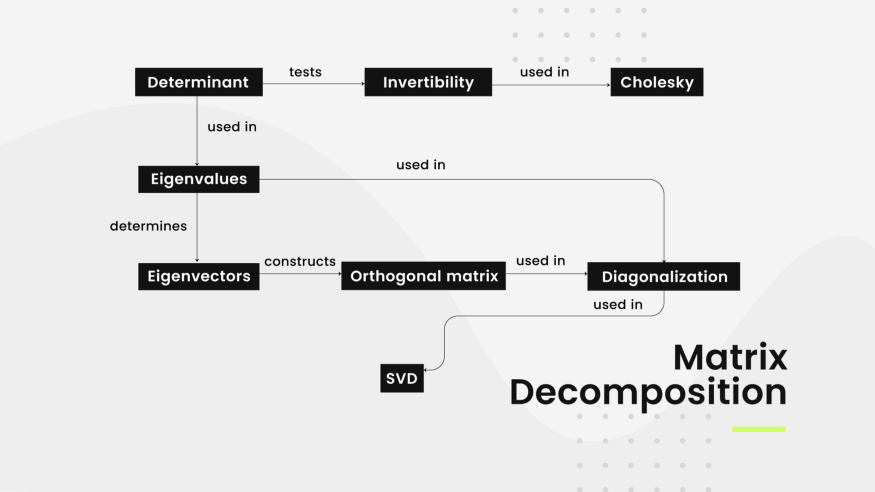
\includegraphics[width=0.9\linewidth,keepaspectratio]{maths4ai2}
% \end{center}

% {\tiny (Ref: The NOT definitive guide to learning math for machine learning - Favio Vazquez)}

% \end{frame}